\begin{figure}
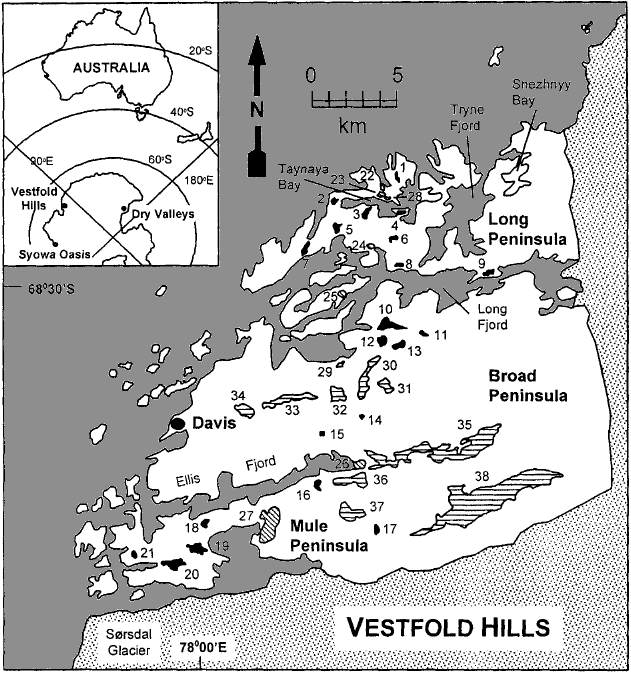
\includegraphics{intro_figures/vestfold_map.png}
\caption[Map of the Vestfold Hills]{A map of the Vestfold Hills showing fjords, bays and lakes (numbered). The Southern Ocean is shown in grey, meromictic lakes coloured in black, seasonally isolated lakes and basins are striped and the continental ice-shelf is stippled. Inset is the position of the Vestfold Hills relative to Australia and to the Antarctic coastal oases. The lakes are: (1) unnamed lake 2, (2) Organic Lake, (3) Pendant Lake, (4) Glider Lake, (5) Ace Lake, (6) unnamed lake 1, (7) Williams Lake, (8) Abraxas Lake, (9) Johnstone Lake, (10) Ekho Lake, (11) Lake Farrell, (12) Shield Lake, (13) Oval Lake, (14) Ephyra Lake, (15) Scale Lake, (16) Lake Anderson, (17) Oblong Lake, (18) Lake McCallum, (19) Clear Lake, (20) Laternula Lake and (21) South Angle Lake. Map image is from \citet{Gibson1999} with some minor modifications.}
\label{fig:vestfold_map}

\end{figure}
